\documentclass[a5paper,11pt]{book}

\title{\textbf{EX VINUM}}
\author{by tsbohc}
\date{}

% {{{ latex

\usepackage[utf8]{inputenc}
\usepackage[russian]{babel}
\usepackage{longtable}
\usepackage[linewidth=0.1pt]{mdframed}
\usepackage{comment}
\usepackage{graphicx}
\usepackage{array}
\usepackage{booktabs}
\usepackage{calc}
\usepackage[table]{xcolor} % table row colors
\usepackage{tabularx} % page width
\usepackage{multicol}
\usepackage{titlesec} % titles customization
\usepackage{CormorantGaramond}
\usepackage{epigraph}
\usepackage{lettrine} % big letters in the beginning of the chapter
\usepackage[margin=0.6in, bottom=0.7in]{geometry}
\usepackage{lettrine} % big letters in the beginning of the chapter
\usepackage{fancyhdr} % page numbers
\usepackage{tocbasic}

%\newmdenv[
%  innerbottommargin=11pt, 
%  innertopmargin=\topskip,
%  font=\itshape,
%  skipabove=\topsep,
%  skipbelow=\topsep
%]{boxed}

\newenvironment{boxed}
{\em\noindent\rule[1ex]{\linewidth}{0.1pt}\linebreak\indent}
{\par\noindent\rule[1ex]{\linewidth}{0.1pt}}

%\newenvironment{boxed}
%    {\em
%    \begin{longtable}{|p{0.9\textwidth}|}
%    \hline
%    }
%    { 
%    \\\hline
%    \end{longtable} 
%    }

% just table things
\definecolor{lightgray}{gray}{0.95}
\definecolor{white}{gray}{1}
\newcolumntype{Y}{>{\centering\arraybackslash}X}
\newcolumntype{Z}{>{\ \ \ }l}
\newcolumntype{P}[1]{>{\centering\arraybackslash}p{#1}}
\setlength{\extrarowheight}{2pt}

% remove epigraph line 
\setlength\epigraphrule{0pt}

% set page numbers at the bottom
\pagestyle{fancy}
\fancyhf{}
\renewcommand{\headrulewidth}{0pt}
\cfoot{\thepage}

% toc 
\setcounter{tocdepth}{1}
\addto\captionsrussian{% Replace "english" with the language you use
  \renewcommand{\contentsname}%
    {Table Of Contents}%
}
\DeclareTOCStyleEntry[
linefill=\bfseries\TOCLineLeaderFill,beforeskip=2pt
]{tocline}{chapter}
\newcommand\chapterprefixintoc[1]{\MakeUppercase{\chaptername}~#1~}

% titles
\titlespacing*{\chapter}{0pt}{12pt plus 4pt minus 4pt}{8pt plus 1pt minus 1pt}
\titlespacing*{\section}{0pt}{12pt plus 4pt minus 4pt}{10pt plus 1pt minus 1pt}
\titlespacing*{\subsection}{0pt}{8pt plus 2pt minus 2pt}{4pt plus 0pt minus 0pt}

\titleclass{\chapter}{straight}

%\definecolor{reddish}{RGB}{76,28,12}
\titleformat{\chapter}
  {\huge\bfseries\scshape} % format
  {}                % label
  {0pt}             % sep
  {} % before-code
  [{\titlerule[0.1pt]}]

\titleformat{\section}
  {\large\bfseries\scshape} % format
  {}                % label
  {0pt}             % sep
  {\Large}          % before-code
  [{\titlerule[0.1pt]}]

\titleformat{\subsection}
  {\large\bfseries\scshape} % format
  {}                % label
  {0pt}             % sep
  {\large}          % before-code

\setlength{\DefaultNindent}{0pt}
\setlength{\DefaultFindent}{6pt}

% }}}

\raggedbottom
\excludecomment{en}
\includecomment{ru}

\begin{document}
\maketitle
\thispagestyle{empty}
\enlargethispage{\baselineskip}
\tableofcontents
\pagebreak

% {{{ intro
\chapter{Introduction}
\begin{multicols}{2}

\begin{en}
\epigraph{\emph{Let your autism stretch far beyond the flowery fields and the foggy mountain peaks}}{--- drunk sorcerer}

\lettrine{E}{x vinum} is a tabletop role-playing game, at the heart of which lie autism and the love for role-playing games, the bounds between which were blurred by wine. That's how it got its name.

The game emphasizes the role-playing aspect of similar titles, while simplifying yet not rejecting the traditional systems.

The setting is classic fantasy world akin to that of D\&D that doesn't strive to be strictly realistic.
\end{en}

\begin{ru}
\epigraph{\emph{Да раскинутся границы твоего аутизма до дальних цветочных полей и дымкой затянутых горных вершин.}}{--- бухой волшебник}

\lettrine{E}{x vinum} -- настольная ролевая игра, в сердце которой лежат любовь к рпг и слабоумие, границы между которыми были размыты вином. Так она и получила свое название.

Игра делает акцент на ролевом аспекте, упрощая, но при этом не отказываясь от признанных систем.

Мир игры -- классический фэнтези в стиле D\&D, не претендующий на строгий реализм.
\end{ru}

\section{Gameplay}
\begin{ru}
Dungeon Master описывает ситуацию. Детали окружения, персонажей. Однако, далеко не вся информация доступна игрокам сразу.

Игроки описывают, что они хотят сделать. Во время боя это происходит по порядку очередности ходов. Вне боя, игроки могут действовать свободно -- один может взламывать сундук, а другой стоять на стороже.

Иногда решить проблему легко, например открыть дверь. В таком случае DM может просто сказать, что дверь открылась, и описать, что лежит за ней. В других случаях, успешность действий игроков определяется бросками костей.

DM описывает результаты действий игроков, и на этом цикл повторяется.

Стоит помнить, что это не компьютерная игра. Действия участников ограничиваются лишь их воображением и фэнтезийной версией законов физики, а минмаксинг может обернуться плачевно.
\end{ru}

\begin{en}
The Dungeon Master describes the situation. The details of the surrounding area, characters, etc. Not all there is to know is available to the players right away.

The players describe what they would like to do. During combat this happens in a strict order. Out of combat, the players can move freely. One of them maybe picking a lock, another standing on guard.

Sometimes, solving a problem is easy, like opening a door. In this case, DM may just say that the door opens and describe what lies beyond. Sometimes, the success of the players' actions depends on dice rolls.

DM describes the results of the players actions, and the cycle continues.

Note that this is not a computer game. The actions of players are constrained only by their imagination and the fantasy version of the laws of physics, and min-maxing doesn't usually end well.
\end{en}

\section{Nota Bene}
\begin{ru}
DM и игроки работают вместе, чтобы создать общий нарратив, а не играют друг против друга.

Что бы ни было написано в правилах, DM всегда имеет последнее слово.

DM должен поощрять изобретательность игроков их способность вживаться в роли, даже если их идеи не реалистичны.

Главная цель не победить, а хорошо провести время в кругу друзей.
\end{ru}

\begin{en}
DM and the players work together to create a narrative, they are not fighting each other.

No matter what is written in the rules, DM always have the last say.

DM must reward players for experimentation and role-playing, even if their ideas are not realistic.

The main goal is not to win, but to have fun with your friends.
\end{en}

\end{multicols}
% }}}

% {{{ races 
\pagebreak
\chapter{Races}
\begin{multicols}{2}

\begin{ru}
\lettrine{Н}{иже} перечислены разумные, игровые расы ex vinum. Полный список существ далеко не закачивается этим разделом.
\end{ru}

\section{Human}
\begin{ru}
Ну, вы поняли. Люди преуспевают во многом, но реже добиваются невероятных результатов. Являются самой многочисленной расой, включающей в себя огромное количество разных культур.
\end{ru}

\begin{en}
Well, you know, the usual. Humans are good at many things, but don't excel at any of them. They are the most diverse and numerous race.
\end{en}

\section{Dwarf}
\begin{ru}
Воспитанные грубой средой обитания и тяжелой работой, Дворфы ценят свое мастерство. Чаще всего они становятся ремеслeнниками или шахтерами. Любят провести вечер пересчитывая свое золото за парой-тройкой-десятком кружек эля.

Невысокого роста. Тучные, мускулистые, с бурым или темным цветом волос, грубоватым голосом и громким смехом.
\end{ru}

\begin{en}
The harsh underground and a lot of hard work. Dwarves cherish their craftsmanship. They often become artisans or miners. They love to spend an evening counting their gold while having a few jugs of ale.

They are short, sturdy, muscular. Brown or dark hair, harsh voice, and thundering laughter.
\end{en}

\section{Elf}
\begin{ru}
Изящные и благоразумные, Эльфы тесно связаны с магией этого мира. Часто становятся писателями или художниками. Большую часть времени проводят наедине с природой и книгами.

Ростом чуть ниже человека. Стройные, светловолосые, часто с голубым или зеленым оттенком глаз. Голоса мелодичны и благозвучны.
\end{ru}

\begin{en}
Graceful and mindful, Elves are tightly connected to the magic of this world. They often become writers or artists. Most of their time they spend alone with nature and books.

Slightly shorter than humans. Slender physique, light hair, blue or green eyes. Melodic voices.
\end{en}

\section{Tiefling}
\begin{ru}
Тифлинги несут за собой бремя своей родословной -- они потомки людей и дьявола. Их полу-демоническое обличие не пробуждают в людях теплых чувств, лишь только косые взгляды. Тифлинги, оказавшиеся в этом мире не по своей воли, делают все, чтобы выжить.

Ростом с человека. Цвета кожи те же, что и у людей, но могут принимать красноватые или фиолетовые оттенки. Длииинный хвост. На голове большие рога. Туманные глаза, темные волосы.
\end{ru}

\begin{en}
Tieflings carry the burden of their ancestry. They are the offspring of the devil and a human. They half-demonic appearances provokes only sharp glares and no compassion. Tieflings were brought into this world against their will, and do everything they can to survive.

Height is around that of a human. The skin color tends to be reddish, violetish, or similar to humans. A long tail, large horns on the top of the head. Misty eyes, dark hair.
\end{en}

\section{Drow}
\begin{ru}
Темные Эльфы произошли от дверней подрасы Эльфов, изгнанных обитать в глубинах земли. Те, что выбираются на поверхность, нередко идут по пути зла, но встречаются и исключения. По большей части становятся путешественниками или наемниками.

Чуть меньше и стройнее своих собратьев. Обладают темным цветом кожи, практически белым цветом волос и бледными глазами с оттенком.
\end{ru}

\begin{en}
  Dark Elves are the ancient sub-race of the traditional Elves. They were condemned to live underground. Those who end up on the surface often follow the path of evil, but there are exceptions. They often become mercenaries or travellers.

Slightly shorter than Elves. Dark, ebony colored skin. Almost white hair, pale eyes.
\end{en}

\section{Aasimar}
\begin{ru}
Азимары подобны Тифлингам в своем происхождении, но в их жилах течет божественная кровь.  Азимары от природы расположены к благотелям, а в своих снах ведут разговоры со своим божеством. Однако, предпочитают не раскрывать свою родословную.

Выше человека. В цветах волосы и кожи встречаются как человеческие, так и более металлические оттенки.
\end{ru}

\begin{en}
Aasimar are similar to Tieflings in their ancestry, only there's divine blood in their veins. They are very likely to become fighters for virtue. In their dreams they speak with their divine father. Aasimar prefer not to reveal their lineage.

Taller than Humans. The skin and hair colors are similar to that of Humans, but may have metallic colors.
\end{en}
\end{multicols}
% }}}

% {{{ roleplaying
\chapter{Roleplaying}
\begin{multicols}{2}
\begin{ru}
\lettrine{К}{ем} будешь ты? Добродушным дворфом с раскатистым смехом, знающим лучшие таверны в городе? Или тифлингом, чьи руки в крови, потому что единственным выбором была смерть?
\end{ru}

\begin{en}
\lettrine{W}{ho} will you be? A cheerful Dwarf with a bellowing laughter who knowns all the best taverns in town? Or a Tiefling, who's hands are covered in blood because the only other choice was death?
\end{en}

\section{Race}
\begin{ru}
Выбор расы влияет не только на физический облик и характеристики, но и ваше положение в мире, а также отношения с другими рассами. Кроме этого, ваша история вытекает из происхождения.
\end{ru}

\begin{en}
Race doesn't only affect physical appearance and character attributes, but also your position in the world, and the relationships with other races. Apart from that, your backstory is directly related to the birthplace.
\end{en}

\section{Age}
\begin{ru}
Некоторые расы, например дворфы и эльфы, живут на несколько сотен лет дольше чем люди. В результате чего имеют другую перспективу на мир.
\end{ru}

\begin{en}
Some races, such as Dwarves and Elves, live a few hundred years older than humans. For this reason, they have a different perception of the world.
\end{en}

\section{Sex}
\begin{ru}
Пол обладает большим влиянием на ваш характер и прошлое. Не все женщины покинув родной дом тут же становятся рыцарями. Рыцарями становятся те женщины, чьим сердцам дорого то, что они хотят защитить.
\end{ru}

\begin{en}
Sex greatly affects your character and past. Not all women can become knights whenever they want. Only those women who have something they want to protect become knights.
\end{en}

\section{Class}
\begin{ru}
Каждый искатель приключений обладает той или иной профессией. Профессия определяет, владаеете ли вы магией или хорошо управляетесь с оружием, и какую роль вам предстоит выполнять в кампании.
\end{ru}

\begin{en}
Every adventurer belongs to a profession. Class determines whether you're proficient with magic or weapons, and what role you'll be filling in your group.
\end{en}

\section{Personality}
\begin{ru}
Личность составляют идеи которые вами движат и недостатки которыми обладаете. Ваши сильные и слабые стороны, ваш характер, и то, как вы ведете себя с другими людьми.
\end{ru}

\begin{en}
Personality is composed of your values and flaws. Your strong and weak sides, your character, and how you behave around other people.
\end{en}

\section{Backstory}
\begin{ru}
Какой была ваша жизнь до начала кампании? Может быть, вас отправили на важное задание, или вовсе изгнали? Как вы преобрели свои навыки и стали своим классом? Что вы хотите защитить или чем желаете овладеть? Есть ли у вас возлюбленный или возлюбленная? Потеряли ли вы старого друга или преследуете врага?
\end{ru}

\begin{en}
What was your life like before the campaign? Maybe you were sent on an important quest or maybe even excommunicated? How did you learn what you know and became your class? What do you want to protect or acquire? Do you have a loved one? Did you lose an old friend or are chasing an enemy?
\end{en}

\section{Appearance}
\begin{ru}
Все, что связано с внешним обликом. Телесложение, цвет кожи, волос, глаз. Шрамы, полученные в бою и татуировки. Детали одежды и украшения, талисманы.
\end{ru}

\begin{en}
Everything that's related to outer appearance. Your physique, the colors of your eyes, skin, hair. The scars you got in past battles and tattoos. The details of your clothing.
\end{en}

\end{multicols}
% }}}

% {{{ character sheet 
\chapter{Character Example}
\setlength{\arrayrulewidth}{0.1pt}
\noindent
\setlength\tabcolsep{0pt}
\def\arraystretch{1.3}
\begin{tabularx}{\linewidth}{@{}YYYYYYYYYYYYY@{}}

  \multicolumn{13}{c}{\large\sc\textbf{Name:}} \\ 
  \multicolumn{13}{c}{\Large\emph{Ailon Dawnguard}} \\ \cline{4-10}

  \addlinespace[0.5cm]

  \multicolumn{6}{c}{\large\sc\textbf{Attributes:}} &
  \multicolumn{1}{c}{} &
  \multicolumn{6}{c}{\large\sc\textbf{Character:}}
  \\ \cline{1-6}

  \multicolumn{2}{c|}{\small\sc\textbf{Str}} &
  \multicolumn{2}{c|}{\small\sc\textbf{Dex}} &
  \multicolumn{2}{c}{\small\sc\textbf{Int}} &
  \multicolumn{1}{c}{} &
  \multicolumn{6}{Z}{\emph{Полу-эльф Волшебник, 24, ж.}}
  \\ \cline{8-13}

  \multicolumn{2}{c|}{\LARGE{+0}} &
  \multicolumn{2}{c|}{\LARGE{+1}} &
  \multicolumn{2}{c}{\LARGE{+2}} &
  \multicolumn{1}{c}{} &
  \multicolumn{6}{Z}{\emph{Сбежала из монастыря чтобы}}
  \\ \cline{1-6} \cline{8-13}

  \multicolumn{2}{c|}{\large{7}} & 
  \multicolumn{2}{c|}{\large{9}} &
  \multicolumn{2}{c}{\large{11}} &
  \multicolumn{1}{c}{} &
  \multicolumn{6}{Z}{\emph{увидеть мир таким, какой он}}
  \\ \cline{8-13}

  \multicolumn{6}{c}{\large\sc\textbf{Stats:}}  &
  \multicolumn{1}{c}{} &
  \multicolumn{6}{Z}{\emph{есть. Хочет стать лучше, но}}
  \\ \cline{1-6} \cline{8-13}

  \multicolumn{3}{c|}{\small\sc\textbf{Max Hp}} &
  \multicolumn{3}{c}{\small\sc\textbf{Gold}} &
  \multicolumn{1}{c}{} &
  \multicolumn{6}{Z}{\emph{боится потерять себя. Веснушки,}}
  \\ \cline{8-13}

  \multicolumn{3}{c|}{\LARGE{46}} &
  \multicolumn{3}{c}{\LARGE{75}} &
  \multicolumn{1}{c}{} &
  \multicolumn{6}{Z}{\emph{русые волосы, невысокий рост.}}
  \\ \cline{1-6} \cline{8-13}
  &  &  &  &  &  &  &  &  &  &  &  & \\
\end{tabularx}

\begin{multicols}{2}

\begin{ru}
Выше живой пример заполненного листа персонажа, на основе моего протагониста \emph{Baldur's Gate 2}.

Игрокам будут выданы дополнительные листки для заметок -- на них можно будет вести заметки и учет своего золота, здоровья, состояний и предметов в инвентаре.

Стоит отметить, что правая колонка -- краткое описание персонажа, на которое я бы опирался, рассказывая его полную историю.
\end{ru}

\begin{en}
Above is the example of my character adapted from \emph{Baldur's Gate 2}.

Players will receive pens and paper for further notes. They can be used to jot down plot points, keep track of health, gold, and equipment.

Note that this column on the right is not the full character description, only a summary.
\end{en}
\end{multicols}
\pagebreak
% }}}

% {{{ rules

\chapter{Rules}
\begin{multicols}{2}

\begin{en}
\lettrine{D}{ie throws} are illustrated with two numbers between the letter 'd'. For example, 3d6 means "throw 3 dice, each with 6 sides". If no further instructions are given, the resulting roll is the sum of all dice.

If there is addition or subtraction afterwards, e.g 2d8+3, 3 is added to the resulting sum of two throws of d8.

At the heart of the role-playing system of ex vinum lies the d12. The reason being, I wanted to shorten the time between something awful and something awesome happening.
\end{en}

\begin{ru}
\lettrine{Б}{роски костей} обозначаются двумя числами через букву d. Например, 3d6 означает три броска кости с 6 сторонами. Если другие указания отсутствуют, подразумевается сумма указанных бросков.

В случае с 2d8+3 к сумме двух бросков d8 прибавляется 3.

В основе ролевой системы ex vinum лежит d12. Это обусловлено желанием добавить динамики традиционной системе d20.
\end{ru}

\section{Ability Scores}
\begin{en}
Character's attributes reflect their physical abilities and mental capacity, and are expressed with numbers from 3 to 12 on average.
\end{en}

\begin{ru}
Атрибуты выражают физические и умственные способности персонажа. Определяются численными значениями, в среднем от 3 до 12.
\end{ru}

\subsection{Strength}
\begin{en}
Determines raw physical ability and constitution, proficiency with heavy weapons. Greatly affects the total number for hit points.
\end{en}

\begin{ru}
Определяет физическую силу и выносливость, умеение обращаться с тяжелым оружием. Имеет большое влияние на общий запас здоровья.
\end{ru}

\subsection{Dexterity}
\begin{en}
Defines character's reflexes and perception, proficiency with light and ranged weapons. Has a minor effect on total health pool.
\end{en}

\begin{ru}
Определяет ловкость и скорость реакции, внимательность, а также умение обращаться с легкий или стрелковым оружием. Слабо влияет на запас здоровья.
\end{ru}

\subsection{Intelligence}
\begin{en}
Indicates background knowledge and charisma, proficiency with intelligence weapons and magic. Doesn't have any effect on health.
\end{en}

\begin{ru}
Определяет ум и сообразительность, фоновые знания, уменее вести разговор, а также навыки в магии. Не влияет на запас здоровья.
\end{ru}

\subsection{Determining Scores}
\begin{en}
For each of the Ability Scores a player rolls 3d4 and adds up the dice. The player can assign the resulting three rolls as he or she wishes.

DM may suggest another way of determining Ability Scores.

Then, racial and other bonuses are applied. Also, the player with the best backstory receives an extra attribute point assigned by the DM.
\end{en}

\begin{ru}
Чтобы определить свои базовые атрибуты, игрок бросает 3d4 и складывает полученные значения. Затем повторяет этот процесс еще два раза. Полученные три ролла игрок распределяет на свое усмотрение.

Перед началом игры DM может предложить свой метод определения атрибутов.

На следующем этапе к характеристикам применяются расовые бонусы. Ирок с лучшей предысторией получает +1 к атрибуту выбранному DM.
\end{ru}

% {{{ race bonuses table
\smallskip
\noindent
\rowcolors{1}{}{lightgray}
\setlength\tabcolsep{0pt}
\begin{tabularx}{\linewidth}{@{}ZYYY@{}}
  \textbf{race} & \textbf{str} & \textbf{dex} & \textbf{int} \\
  \hline
  dwarf     & +2 & -1 &    \\
  elf       & -1 &    & +2 \\
  tiefling  &    & +2 & -1 \\
  %duergar   & +1 & +1 & -1 \\
  drow      & -1 & +1 & +1 \\
  aasimar   & +1 & -1 & +1
\end{tabularx}
\smallskip
% }}}

\begin{en}
Humans receive +1 to any Ability Score of their choosing.
\end{en}

\begin{ru}
Люди получают +1 к любому выбранному атрибуту.
\end{ru}

\subsection{Hit Points}
\begin{en}
The total health pool of character is determined by
\end{en}

\begin{ru}
Максимальный запас здоровья расчитывается по следующей формуле:
\end{ru}
\textbf{6 × Strength + 2 × Dexterity}.

\subsection{Score Modifiers}
\begin{en}
Score Modifiers are used to show how well or how badly a character is proficient with a skill. They play an integral part in determining how successful an action is.

High Ability Scores result in positive Score Modifiers, low -- in negative.
\end{en}

\begin{ru}
Модифаеры используются чтобы подчеркнуть, насколько хорошо или плохо персонаж владеет тем или иным навыком, и участвуют в подсчете роллов.

Высокие значения атрибутов пораждают положительные моды, низкие -- отрицательные.
\end{ru}

% {{{ modifiers table
\smallskip
\noindent
\rowcolors{1}{}{lightgray}
\setlength\tabcolsep{0pt}
\begin{tabularx}{\linewidth}{@{}YYYY@{}}
  \textbf{attr} & \textbf{mod} & \textbf{attr} & \textbf{mod} \\
  \hline
  1-2 & -3 & 9-10 & +1 \\
  3-4 & -2 & 11-12 & +2 \\
  5-6 & -1 & 13-14 & +3 \\
  7-8 & -0 & 15-16 & +4
\end{tabularx}
% }}}

\section{Ability Checks}
\begin{en}
If there's a chance of a player's action failing, DM will ask him to perform an Ability Check.

The player must throw a d12 and add relevant Modifiers to the roll. If the final roll is equal or higher than the Difficulty Class set by DM, the action succeeds.

%Saving Throws, meaning rolling for a chance to resist damage, are also included in this mechanic and function the same way. DM will ask the player to roll for an Ability Check when a Saving Throw is valid.
\end{en}

\begin{ru}
В случае, когда действие игрока имеет шанс на провал, DM просит его сделать ролл на проверку аттрибута.

Игрок просает d12 и добавляет к нему модифаер, указанный DM. Если итоговый ролл равен или выше сложности, установленной DM, то действие успешно.
\end{ru}

\subsection{Advantage}
\begin{en}
There can be a case, where a player gains an Advantage when performing a certain action. This means that during an Ability Check the player throws 2d12 instead of one, and picks the highest roll. Remember to add your Modifiers to it.
\end{en}

\begin{ru}
У игрока может быть преимущество в выполнении того или иного действия. В этом случае, во время ролла на проверку атрибута игрок делает бросает 2d12 и выбирает наибольший ролл. Не забывайте прибавлять свои модифаеры.
\end{ru}

\subsection{Assisting}
\begin{en}
A player may assist another by rolling a d12 beforehand and adding a relevant Modifier. If he rolls more than 6, the player performing an action gains an Advantage.
\end{en}

\begin{ru}
Один из игроков можем помочь другому в проверке атрибута, предварительно кинув d12. Если ролл с бонусами больше 6, игрок, которому помогают получает преимущество.
\end{ru}

\section{Out of Combat}
\begin{en}
At the beginning of the campaign the players may want to elect someone to be the leader of the group.

Out of combat players may move freely, with the party leader speaking for the rest of the party, for example: "We proceed further into the hallway", etc.

There is no specific order of action when out of combat.
\end{en}

\begin{ru}
В начале кампании игроки могут избрать лидера группы.

Вне боя игроки передвигаются свободно, действия группы может описывать ее лидер, например: "Мы двигаем дальше по коридору" и т.д

и взаимодействуют с окружением без какого либо установленного порядка.
\end{ru}

\section{In Combat}
\begin{en}
Combat consists of rounds. During each round, every character on the battlefield performs a single action.
\end{en}

\begin{ru}
Бои проходят по раундам. За один раунд каждый участник боя ходит один раз.
\end{ru}

\subsection{Initiative}
\begin{en}
If the players ambush their enemies, they can determine the turn order themselves.

If the players are ambushed, they roll for Initiative. The turn order is based on a Dexterity based Ability Check, from highest to lowest.
\end{en}

\begin{ru}
Если игроки устраивают засаду, у них есть возможность установить порядок ходов между собой.

В противном случае, игроки делают ролл на инициативу, подобный роллу на проверку ловкости. Порядок ходов выстраивается от большего к меньшему.
\end{ru}

\subsection{Vision}
\begin{en}
The players can only interact with objects their characters are able to see.

Vision more or less follows the rules of logic. It's very hard to hind successfully if someone is starting you dead in the eyes.
\end{en}

\begin{ru}
Игроки могу взаимодействовать только с теми объектами, которые видят их персонажи.

Все подчинается логике, например, очень трудно успешно спрятаться когда кто-то смотрит на тебя в упор.
\end{ru}

\subsection{Rolling}
\begin{en}
The success of each action is determined by rolling a d12 without any Modifiers.

1 means critical failure, where everything goes awry and somebody gets hurt. 2 is usually a miss and not much else.

Higher values provide good results, with 12 being a critical success, where you learn as much as possible, deal the most damage, etc.
\end{en}

\begin{ru}
Успешность каждого действия в бою определяется одним роллом d12 без модифаеров.

1 означает критический провал, когда все идет не по плану. 2 обычно промах и ничего больше.

Высокие значения дают лучшие результаты. 12 означает критический успех, когда ты узнаешь все что можно узнать или наносишь наибольший урон.
\end{ru}

\subsection{Damage}
\begin{en}
The damage is equal to the roll we just discussed, with the addition of relevant Modifiers. On critical successes, blows deal double the damage.
\end{en}

\begin{ru}
Урон, наносимый атакой или заклинанием равен сумме ролла о котором мы только что говорили и соответствующего модифаера. В случае критического успеха урон удваивается.
\end{ru}

\subsection{Opportunity Attacks}
\begin{en}
If a character is engaged in melee combat with another character and attempts an escape, he will receive an Attack of Opportunity.

There are exceptions to this rule. The success of the escape is determined by an Ability Check. On critical success, the character fully avoids damage. Or if the escaping character using a certain ability.
\end{en}

\begin{ru}
Если персонаж, находясь в ближем бою с другим персонажем делает попытку сбежать, по нему проходит атака возможности.

У данной ситуации есть исключения: критический успех побега, определенный роллом на проверку аттрибута, или использование особого умения.
\end{ru}

\subsection{Death}
\begin{en}
Once a player character's health pool reaches zero, they are knocked unconscious, additionally, their Strength is reduced by 2. A friendly character can then spend an action to help them get up. If a character's Strength reaches 0, they die permanently (and play as a dog, probably).

Very often NPCs die permanently once they run out of hit points.
\end{en}

\begin{ru}
  Когда у персонажа игрока заканчивается здоровье, их вырубает. Кроме этого, их сила снижается на 2. Другой персонаж может помочь лежащему придти в чувства, потратив на это свой ход. Если сила игрока опускается до 0, они умирают перманентно.
\end{ru}

\section{Resting}
\begin{en}
During the course of the campaign, the players will have the ability to set up camp and rest. The quality of the rest depends on their role-playing actions. Rest recovers lost health points.

To rest well, the players need to have dinner, properly set up camp, and tell a few stories around the fire.
\end{en}

\begin{ru}
На протяжение кампании у игроков будет возможность разбить лагерь и отдохнуть. Качество отдыха определяется ролевой игрок персонажей. Отдых восстанавливает игрокам здоровье.

Для хорошего отдыха необходимо хорошо поесть, обустроить лагерь и рассказать пару историй у костра.
\end{ru}

\end{multicols}
% }}}

% {{{ equipment
\pagebreak
\chapter{Equipment}

\noindent
\rowcolors{1}{}{lightgray}
\setlength\tabcolsep{0pt}
\setlength\LTleft{0pt}
\setlength\LTright{0pt}
\begin{longtable}{p{0.4\textwidth}P{0.1\textwidth}p{0.4\textwidth}P{0.1\textwidth}}
  \textbf{\ \ \ name}
  & \textbf{price}
  & \textbf{\ \ \ name}
  & \textbf{price}
  \\
  \hline
  \ \ \ зелье здоровья                  &  25g &
  \ \ \ зелье разговора с животными     &  10g \\
  \ \ \ зелье ночного зрения            &  10g &
  \ \ \ зелье подводного дыхания        &  10g \\
  \ \ \ зелье паучьих ног               &  25g &
  \ \ \ фляска кислоты                  &  10g \\
  \ \ \ фляска вечной мерзлоты          &  10g &
  \ \ \ фляска дымовой завесы           &   5g \\
  \ \ \ фляска света                    &  10g &
  \ \ \ порошок усыпления               &   5g \\
  \ \ \ горсть пороха                   &   5g &
  \ \ \ палатка                         &  10g \\
  \ \ \ котел                           &   5g &
  \ \ \ огниво                          &   5g \\
  \ \ \ соль и перец                    &   2g &
  \ \ \ бинты                           &  15g \\
  \ \ \ бутылка виски                   &   3g &
  \ \ \ отмычки                         &   5g \\
  \ \ \ крюк                            &   5g &
  \ \ \ железные колючки                &   5g \\
  \ \ \ зеркало                         &  10g &
  \ \ \ факел                           &   3g \\
  \ \ \ веревка                         &   5g &
  \ \ \ мыло                            &   1g \\
  \ \ \ лопата                          &   5g &
  \ \ \ топорик                         &   5g \\
  \ \ \ кирка                           &   5g &
  \ \ \ музыкальный инструмент          &   5g
  \\

\end{longtable}

\begin{ru}
По поводу наличия предметов неуказанных выше можно спросить у торговца.
\end{ru}

\begin{en}
You can ask the merchant for the availablity of an item you don't see above.
\end{en}
% }}}

% {{{ print only

\pagebreak
\rowcolors{1}{}{}

\noindent
\setlength\tabcolsep{0pt}
\def\arraystretch{1.3}
\begin{tabularx}{\linewidth}{@{}YYYYYYYYYYYYY@{}}

  \multicolumn{13}{c}{\large\sc\textbf{Name:}} \\ 
  \multicolumn{13}{c}{\Large\emph{}} \\ \cline{4-10}

  \addlinespace[0.5cm]

  \multicolumn{6}{c}{\large\sc\textbf{Attributes:}} &
  \multicolumn{1}{c}{} &
  \multicolumn{6}{c}{\large\sc\textbf{Character:}}
  \\ \cline{1-6}

  \multicolumn{2}{c|}{\small\sc\textbf{Str}} &
  \multicolumn{2}{c|}{\small\sc\textbf{Dex}} &
  \multicolumn{2}{c}{\small\sc\textbf{Int}} &
  \multicolumn{1}{c}{} &
  \multicolumn{6}{Z}{\emph{}}
  \\ \cline{8-13}

  \multicolumn{2}{c|}{\LARGE{}} &
  \multicolumn{2}{c|}{\LARGE{}} &
  \multicolumn{2}{c}{\LARGE{}} &
  \multicolumn{1}{c}{} &
  \multicolumn{6}{Z}{\emph{}}
  \\ \cline{1-6} \cline{8-13}

  \multicolumn{2}{c|}{\large{}} & 
  \multicolumn{2}{c|}{\large{}} &
  \multicolumn{2}{c}{\large{}} &
  \multicolumn{1}{c}{} &
  \multicolumn{6}{Z}{\emph{}}
  \\ \cline{8-13}

  \multicolumn{6}{c}{\large\sc\textbf{Stats:}}  &
  \multicolumn{1}{c}{} &
  \multicolumn{6}{Z}{\emph{}}
  \\ \cline{1-6} \cline{8-13}

  \multicolumn{3}{c|}{\small\sc\textbf{Max Hp}} &
  \multicolumn{3}{c}{\small\sc\textbf{Gold}} &
  \multicolumn{1}{c}{} &
  \multicolumn{6}{Z}{\emph{}}
  \\ \cline{8-13}

  \multicolumn{3}{c|}{\LARGE{}} &
  \multicolumn{3}{c}{\LARGE{}} &
  \multicolumn{1}{c}{} &
  \multicolumn{6}{Z}{\emph{}}
  \\ \cline{1-6} \cline{8-13}
  &  &  &  &  &  &  &  &  &  &  &  & \\
\end{tabularx}

\vspace{40pt}

\noindent
\setlength\tabcolsep{0pt}
\def\arraystretch{1.3}
\begin{tabularx}{\linewidth}{@{}YYYYYYYYYYYYY@{}}

  \multicolumn{13}{c}{\large\sc\textbf{Name:}} \\ 
  \multicolumn{13}{c}{\Large\emph{}} \\ \cline{4-10}

  \addlinespace[0.5cm]

  \multicolumn{6}{c}{\large\sc\textbf{Attributes:}} &
  \multicolumn{1}{c}{} &
  \multicolumn{6}{c}{\large\sc\textbf{Character:}}
  \\ \cline{1-6}

  \multicolumn{2}{c|}{\small\sc\textbf{Str}} &
  \multicolumn{2}{c|}{\small\sc\textbf{Dex}} &
  \multicolumn{2}{c}{\small\sc\textbf{Int}} &
  \multicolumn{1}{c}{} &
  \multicolumn{6}{Z}{\emph{}}
  \\ \cline{8-13}

  \multicolumn{2}{c|}{\LARGE{}} &
  \multicolumn{2}{c|}{\LARGE{}} &
  \multicolumn{2}{c}{\LARGE{}} &
  \multicolumn{1}{c}{} &
  \multicolumn{6}{Z}{\emph{}}
  \\ \cline{1-6} \cline{8-13}

  \multicolumn{2}{c|}{\large{}} & 
  \multicolumn{2}{c|}{\large{}} &
  \multicolumn{2}{c}{\large{}} &
  \multicolumn{1}{c}{} &
  \multicolumn{6}{Z}{\emph{}}
  \\ \cline{8-13}

  \multicolumn{6}{c}{\large\sc\textbf{Stats:}}  &
  \multicolumn{1}{c}{} &
  \multicolumn{6}{Z}{\emph{}}
  \\ \cline{1-6} \cline{8-13}

  \multicolumn{3}{c|}{\small\sc\textbf{Max Hp}} &
  \multicolumn{3}{c}{\small\sc\textbf{Gold}} &
  \multicolumn{1}{c}{} &
  \multicolumn{6}{Z}{\emph{}}
  \\ \cline{8-13}

  \multicolumn{3}{c|}{\LARGE{}} &
  \multicolumn{3}{c}{\LARGE{}} &
  \multicolumn{1}{c}{} &
  \multicolumn{6}{Z}{\emph{}}
  \\ \cline{1-6} \cline{8-13}
  &  &  &  &  &  &  &  &  &  &  &  & \\
\end{tabularx}

% }}}

% {{{ campaign

\pagebreak
\chapter{Bad Water}

\begin{multicols}{2}
The part is recruited to escort a supply wagon, it gets raided. The part and the coachman reach the destination, get paid very little. The small village they arrive it recently became known for its incredibly potent ale. In reality, there's a cult in the catacomb underneath that poisons the water to steal souls of those who drink it, and restore the physical form of an ancient being.

\section{Prologue}
Empty tavern in the middle of nowhere. No alcohol.

\begin{boxed}
Дело клонится к вечеру, небо затягивают облака, ночь надвигается темная.

По воли случая, таинственных обстоятельств или какой-то верховной силы трое незнакомцев в поисках ночлега прибывают в таверну на опушке леса. По обоим сторонам от крыльца тянется дорога и через какое-то время скрывается за деревьями. Настоящая глушь. Заведение небольшое, построено давно, крыша течет, повсюду пыль.

За стойкой на стуле стоит хозяин со скучающим видом. У камина похрапывает темный эльф, лицо его закрывает соломеная шляпа. Других посетителей нет. К вам обращается хозяин -- Милости просим, чего желаете?
\end{boxed}

\subsection{hook}
The tavernkeep recruits the party to escort a supply cart and bring him booze.

\begin{boxed}
Выпивки уже два дня нет, вот все и разбежались. А послать некого, неуютно нынче в лесу.

*осматривает вас* А вы знать, путешественники? Небось народ удалый.

Неподалеку деревня, с недавнего времени прославилась своим элем. До нее рукой подать, к закату вернетесь. Привезете мне партию, отблагодарю честной монетой. Коли отправитесь сегодня, заплачу вдвойне, а то таверна совсем не таверна без выпивки.
\end{boxed}

Enter Ghinchi

\begin{boxed}
Эй, Гинчи! ГИНЧИ!! -- дроу у камина громко всхрапывает -- Иди запрягай лошадь, поедите в Кельт за выпивкой. Эльф поднимается, но ворчит что-то себе под нос и выходит через заднюю дверь. -- Он подождет вас снаружи. Хорошего пути.
\end{boxed}

Outside

\begin{boxed}
Гинчи стоит рядом с повозкой явно повидавшей свет и ворошит лошадь за гриву -- "ути ты моя пташка". заметив вас, он поворачивается к вам. в зубах у него травинка, на голове все та же соломенная шляпа, а на шее висит наконечник стрелы.

-- why are you here -- да так, проездом, думал подзаработать а у старого хрыча *он говорит это с ухмылкой, без зла* закончилась вся выпивка

-- who are you -- ну теперь я колешу по континенту, продаю всякую всячину.

-- past -- раньше был наемником, но когда напарника убили решил бросить

-- arrowhead -- это так, талисман. этой стрелой убили напарника. прям промешь глаз *взгляд его застывает*
\end{boxed}

If PC ask him what he has for sale give them a printout. Each of the players can get one item off of Ghinci for half the price.

\begin{boxed}
Дорога непростая, вам не помешало бы закупиться. "Скидки новым покупателям", подмигивает он.

===

Ну что, в путь?
\end{boxed}

\subsection{Escort}

\begin{boxed}
Вы в пути около часа, начинает смеркаться

Откуда-то неподалеку доносится волчий вой. Гинчи бросает на Наташу обеспокоинный взгляд.

Справа шуршат кусты и на дорогу выбегают три волка. Бой начался
\end{boxed}

ENCOUNTER: 2-3 wolves

\begin{boxed}
Расправившись с волками, вы продолжаете путь. Становится уже совсем темно и ничего не видно даже на пару шагов вперед.

=====

Из всепоглощающей темноты появляется человек в темной одежде, он стоит облокатившись к стволу дерева.

Приветствую, добрые путники. Чего везете? *легким движением он откидывает край камзола, на поясе у него поблескивает кинжал*

===

Мои напарники вон там в кустах *он указывает куда-то в темную чащу*
\end{boxed}

ENCOUNTER: 2 bandits

\section{Kelt}
A small village with fields surrounding it. Notable is only a tavern and a brewery. A couple of random houses.

\begin{boxed}
Светает, погода стоит ясная, на небе нет ни облачка, ночь вас вымотала. По сторонам дороги расстилаются золотые солодовые поля. Люди, двигаясь рядом, одновременно взмахивают косами, но песни не слышно.

Вы прибываете в деревнью.

Картина перед вами скромная: несколько домов сложенных из бревен, а среди них примечательна только таверна. Гинчи останавливает повозку близ таверны, слезает с места кучера и закуривает.

Ну, теперь не грех и выпить, проверить слухи, а?
\end{boxed}

\section{Tavern}
Bear's claw, lots of people, loud.

\subsection{Upstairs}

\begin{boxed}
На вывеске таверны название -- "Коготь Медведя". Изнутри доносятся громкие разговоры и частые раскаты смеха.

Помещение хорошо освещено, стены бревенчатые. несколько штук круглых столов, барная стойка. на стене лапа медведя.

Вы слышите голос, "Присаживайтесь, присаживайтесь мои хорошие!"

К вам направляется хозяин таверны, добродушный на вид дворф.  Подойдя к вам он прищуривается и говорит, "да вам неплохо бы вздремнуть, у нас как раз внизу свободная комната"
\end{boxed}

\subsection{Drinks}

give players a menu. ask if they want to say toasts

\begin{boxed}
сказать, что выпивка хороша, значит ничего не сказать.

Наталья -- ты чувствуешь как что-то мягкое касается твоей ноги.
\end{boxed}

Ghinchi orders one more drink and downs it immediately. Shortly after he forgets a  party member.

\begin{boxed}
"Хозяин, еще одну!", кричит Гинчи. Он залпом выбивает пинту. Ух давно я так ни с кем не сидел *он делает паузу и со стеклянным выражением лица смотрит тебе в глаза* а ты вообще кто?
\end{boxed}

\subsection{Downstairs}

\begin{boxed}
На полу ковер, постелей всего две. Одному из вас придется спать на полу.
\end{boxed}
 
TREASURE: Ghinci gives players his luchy coin.

\section{Juro}
\textbf{per mid} в траве свернувшись в клубочек лежит черный кот. в сумерках его почти не видно. его глаза поблескивают и направлены на вас

\begin{boxed}
  ... Для остальных это звучит как мяуканье. 

  Бля, чувак, ты меня напугал.

  Слушай, тут что-то неладное, люди стали вести себя странно, а по ночам я вижу как вокруг колодца ошиваются странные типы.
\end{boxed}

\subsection{Well}
\begin{boxed}
  По дороге у вас ногами у вас шуршит трава

  Перед вам обычный деревенский колодец, с виду ничего необычного. Глубокий, внизу вода.
\end{boxed}

\section{Act II}

\subsection{Descent}

\begin{boxed}
Вода жутко холодная, такая, что сковывает легкие. И как будто дурманит, мысли начинают путаться и как будто покидать вас. Долго вы не продержитесь.
\end{boxed}

Do random \textbf{con checks}. There's a hole punched through the bricks somewhere under the water around the middle. The hole is also full of water.

\begin{boxed}
Тунель идет вбок, потом вниз, потом снова вбок, потом снова вниз, у вас перехватывает дыхание, снова вбок и наконец назад и вверх. Вы выплываете на поверхность и жадно глотаете воздух. Кругом стоит абсолютная тьма, воздух холодный, сырой. Воцарившуюся тишину прерывают лишь звуки падения капель воды. Вы промокли до нитки и думать о законах сообщающихся сосудов у вас просто нет сил. 
\end{boxed}

\subsection{1: Cave}
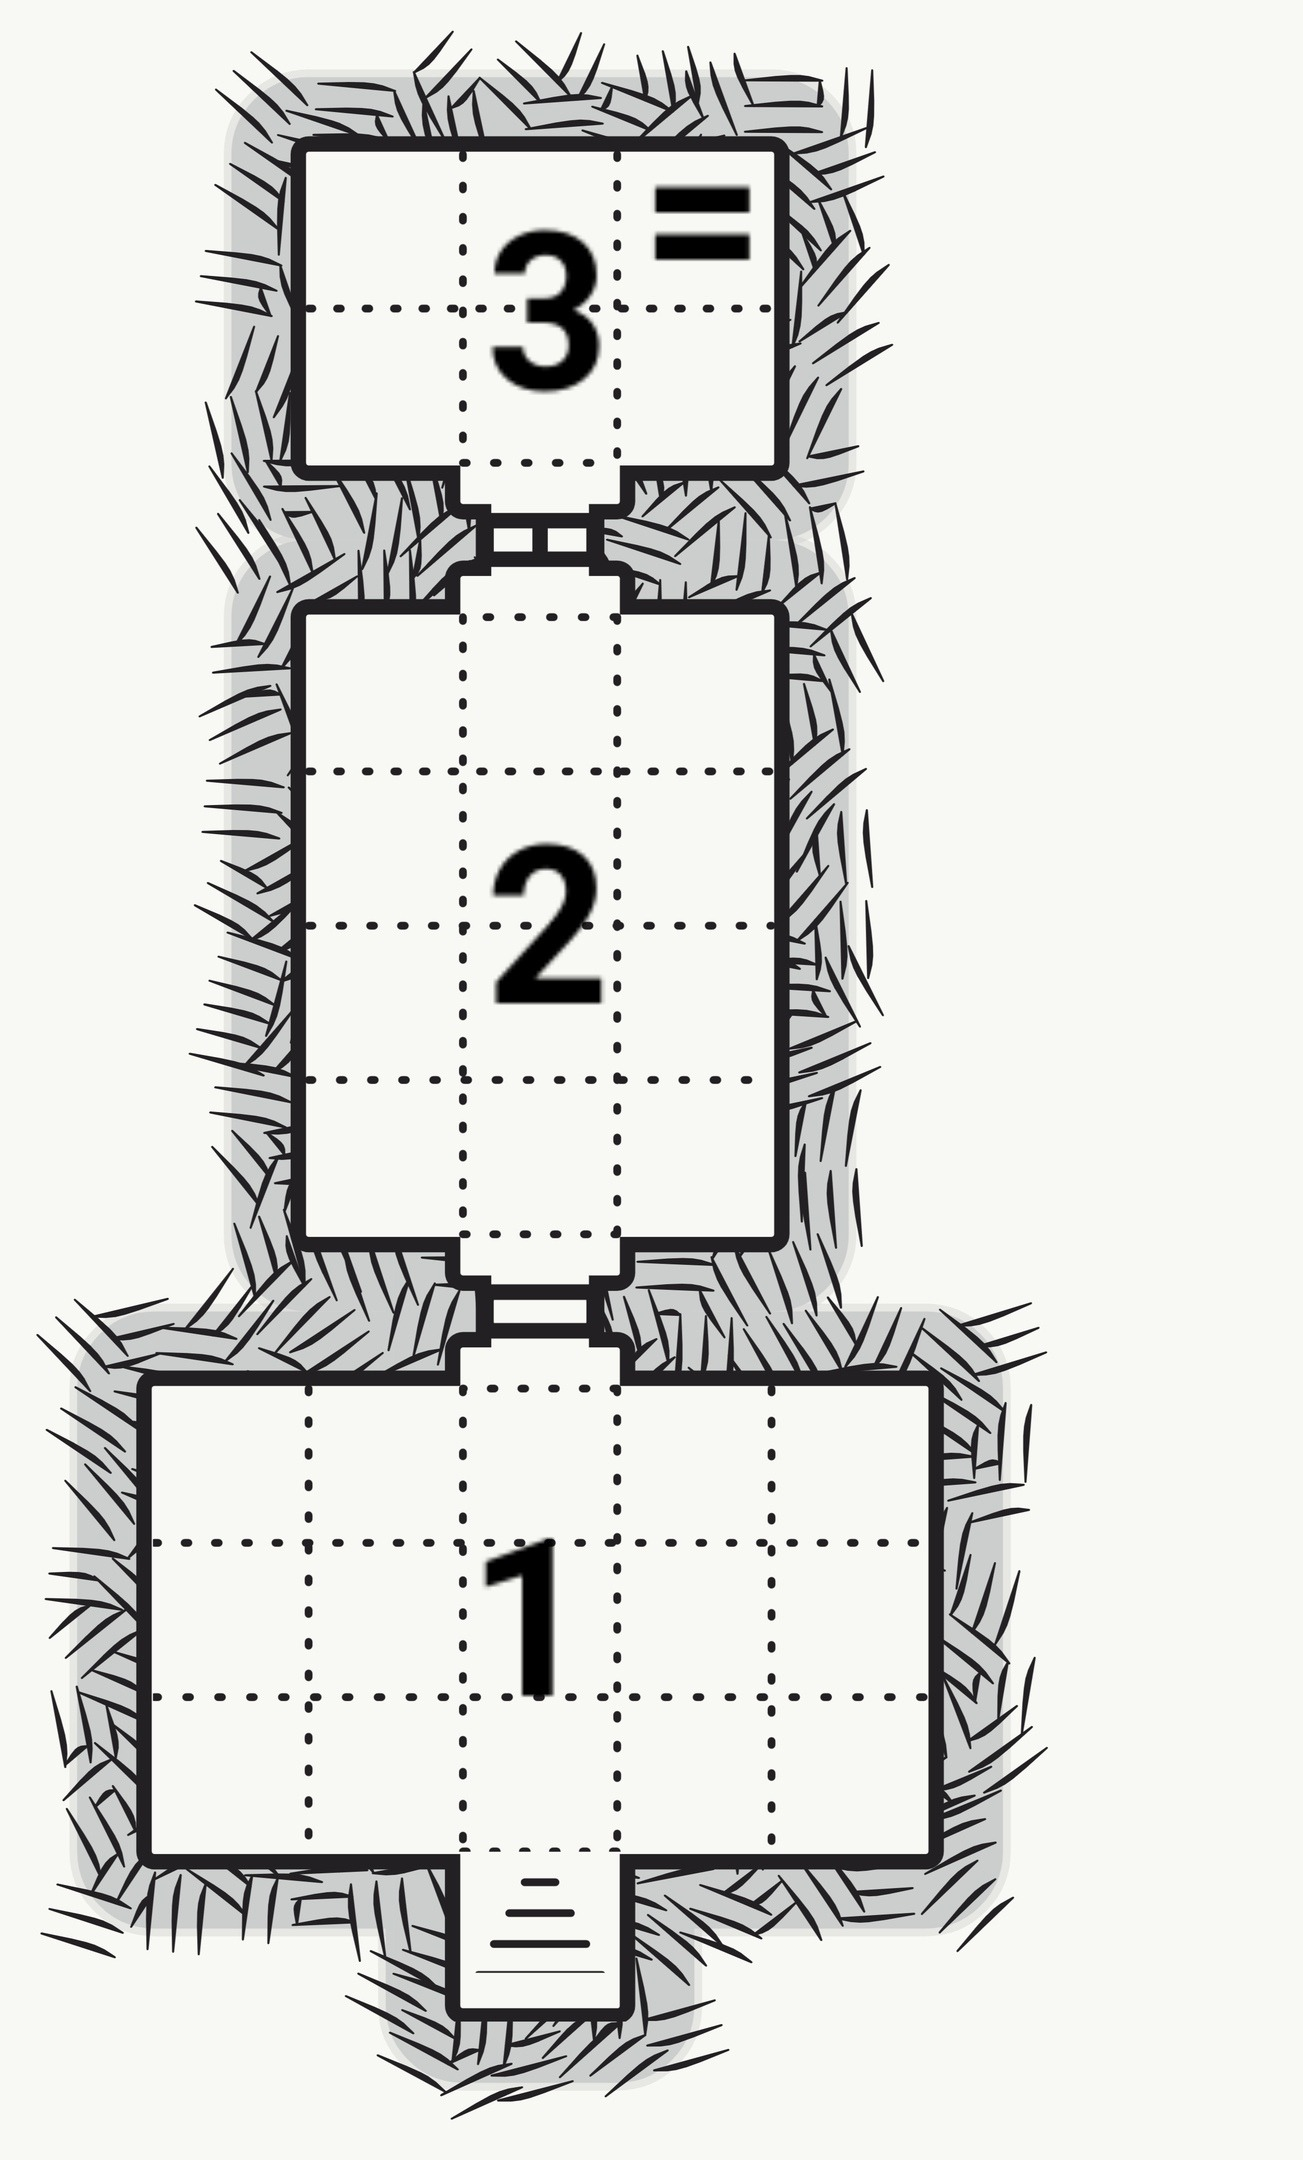
\includegraphics[width=0.5\textwidth]{1}

\begin{enumerate}
\item По земле слабым потоком течет багровая жидкость. Сталагмиты/сталагтиты Впереди во мраке раздается шорох ENCOUNTER: a few big bad rats
\item На земле лужа багрового оттенка, капли которые вы слышали ранее была не вода, а кровь которая просачивается через отверствия в железном потолке.
\item Эта комната чуть выше, у стены справа стоит деревянная лестница которая уходит в потолок через дыру
\end{enumerate}

\subsection{2: Chasm}

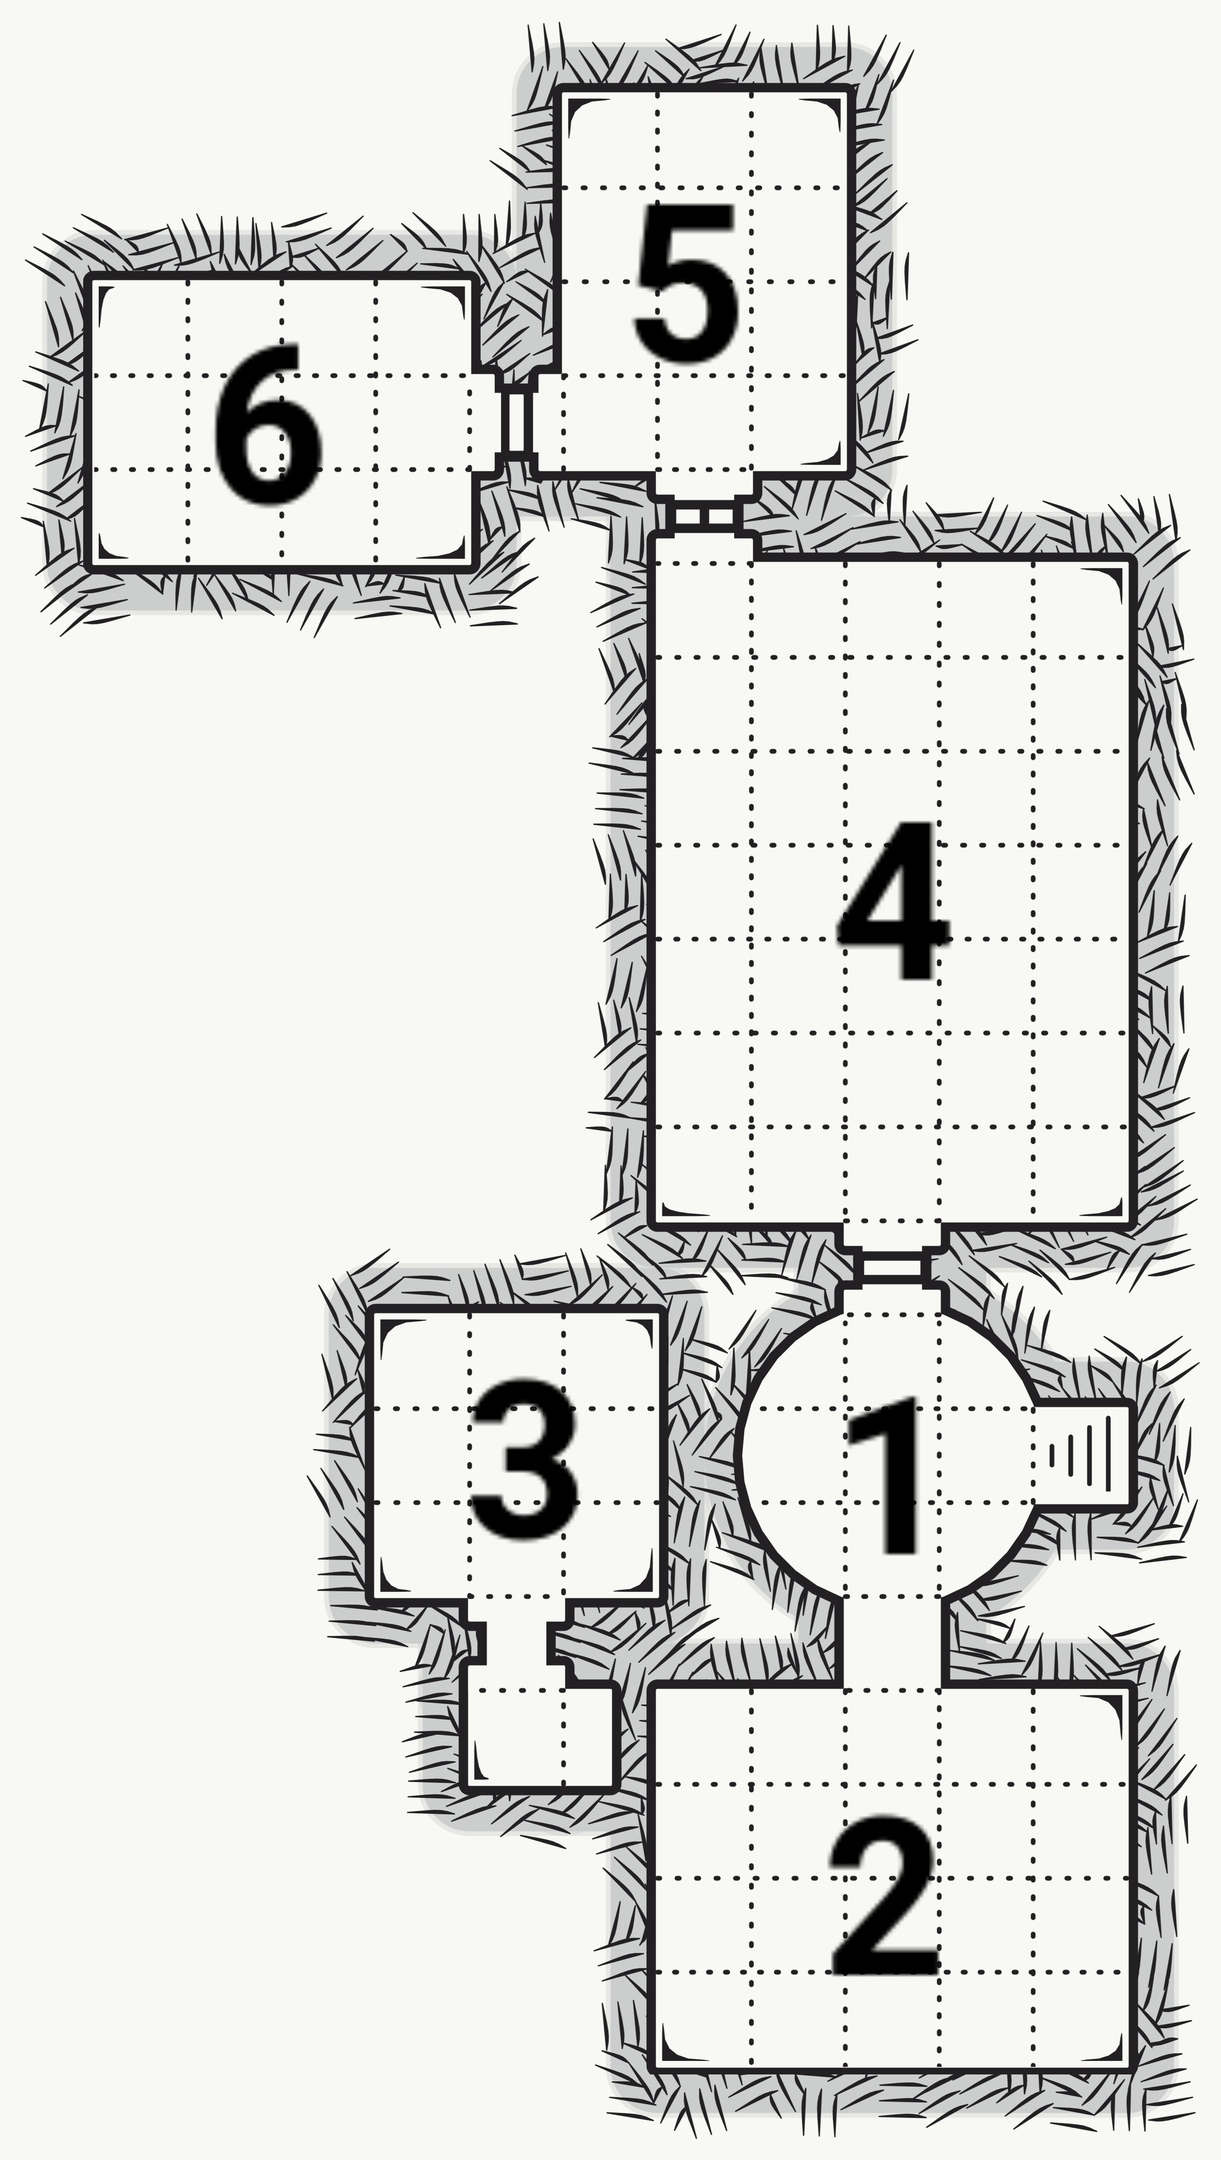
\includegraphics[width=0.5\textwidth]{2}

\begin{enumerate}
\item Стены из каменного кирпича, на них растет мох кровавого цвета, кое-где на земле грибы, селитра.
\item В комнате кое-где обвалился потолок, валяется какая-то деревянная рухлядь вроде прогнивших досок.
\item SECRET!! стена загорожденная рухлядью достаточно слабая чтобы ее проломить. В комнате стоит закрытый сундук. В сундуке TREASURE пара ботинков и записка. 

\begin{boxed}
  Оставил их на случай если ты опять ("как придурок" зачерикано) свалишься в колодец. Ты знаешь что делать 

-- KM
\end{boxed}

\item Впереди у двери на стене горит факел. Прямо после закрытой двери на входе обрыв. CON MID. Если все совсем плохо, пусть обнаружат крюк на потолке.
\item Из-за приоткрытой двери слева слышен храп. Впереди лестница вниз, перед ней TRAP ловушка шипованный капкан
\item В комнате факел, стол, стул, матрас на полу, колокол на стене. На кровате спит человек. Еду ему приносят, он практически пленник. 

\begin{boxed}
-- who -- "Я Грег. Ночью я шел домой через поле, меня поймали, посадили сюда и сказали чтобы я звонил если что-то случится." 

-- what do you know -- "А там наверху эти... штуки, я слишком боюсь чтобы подняться"
\end{boxed}
\end{enumerate}

\subsection{3: Chamber}
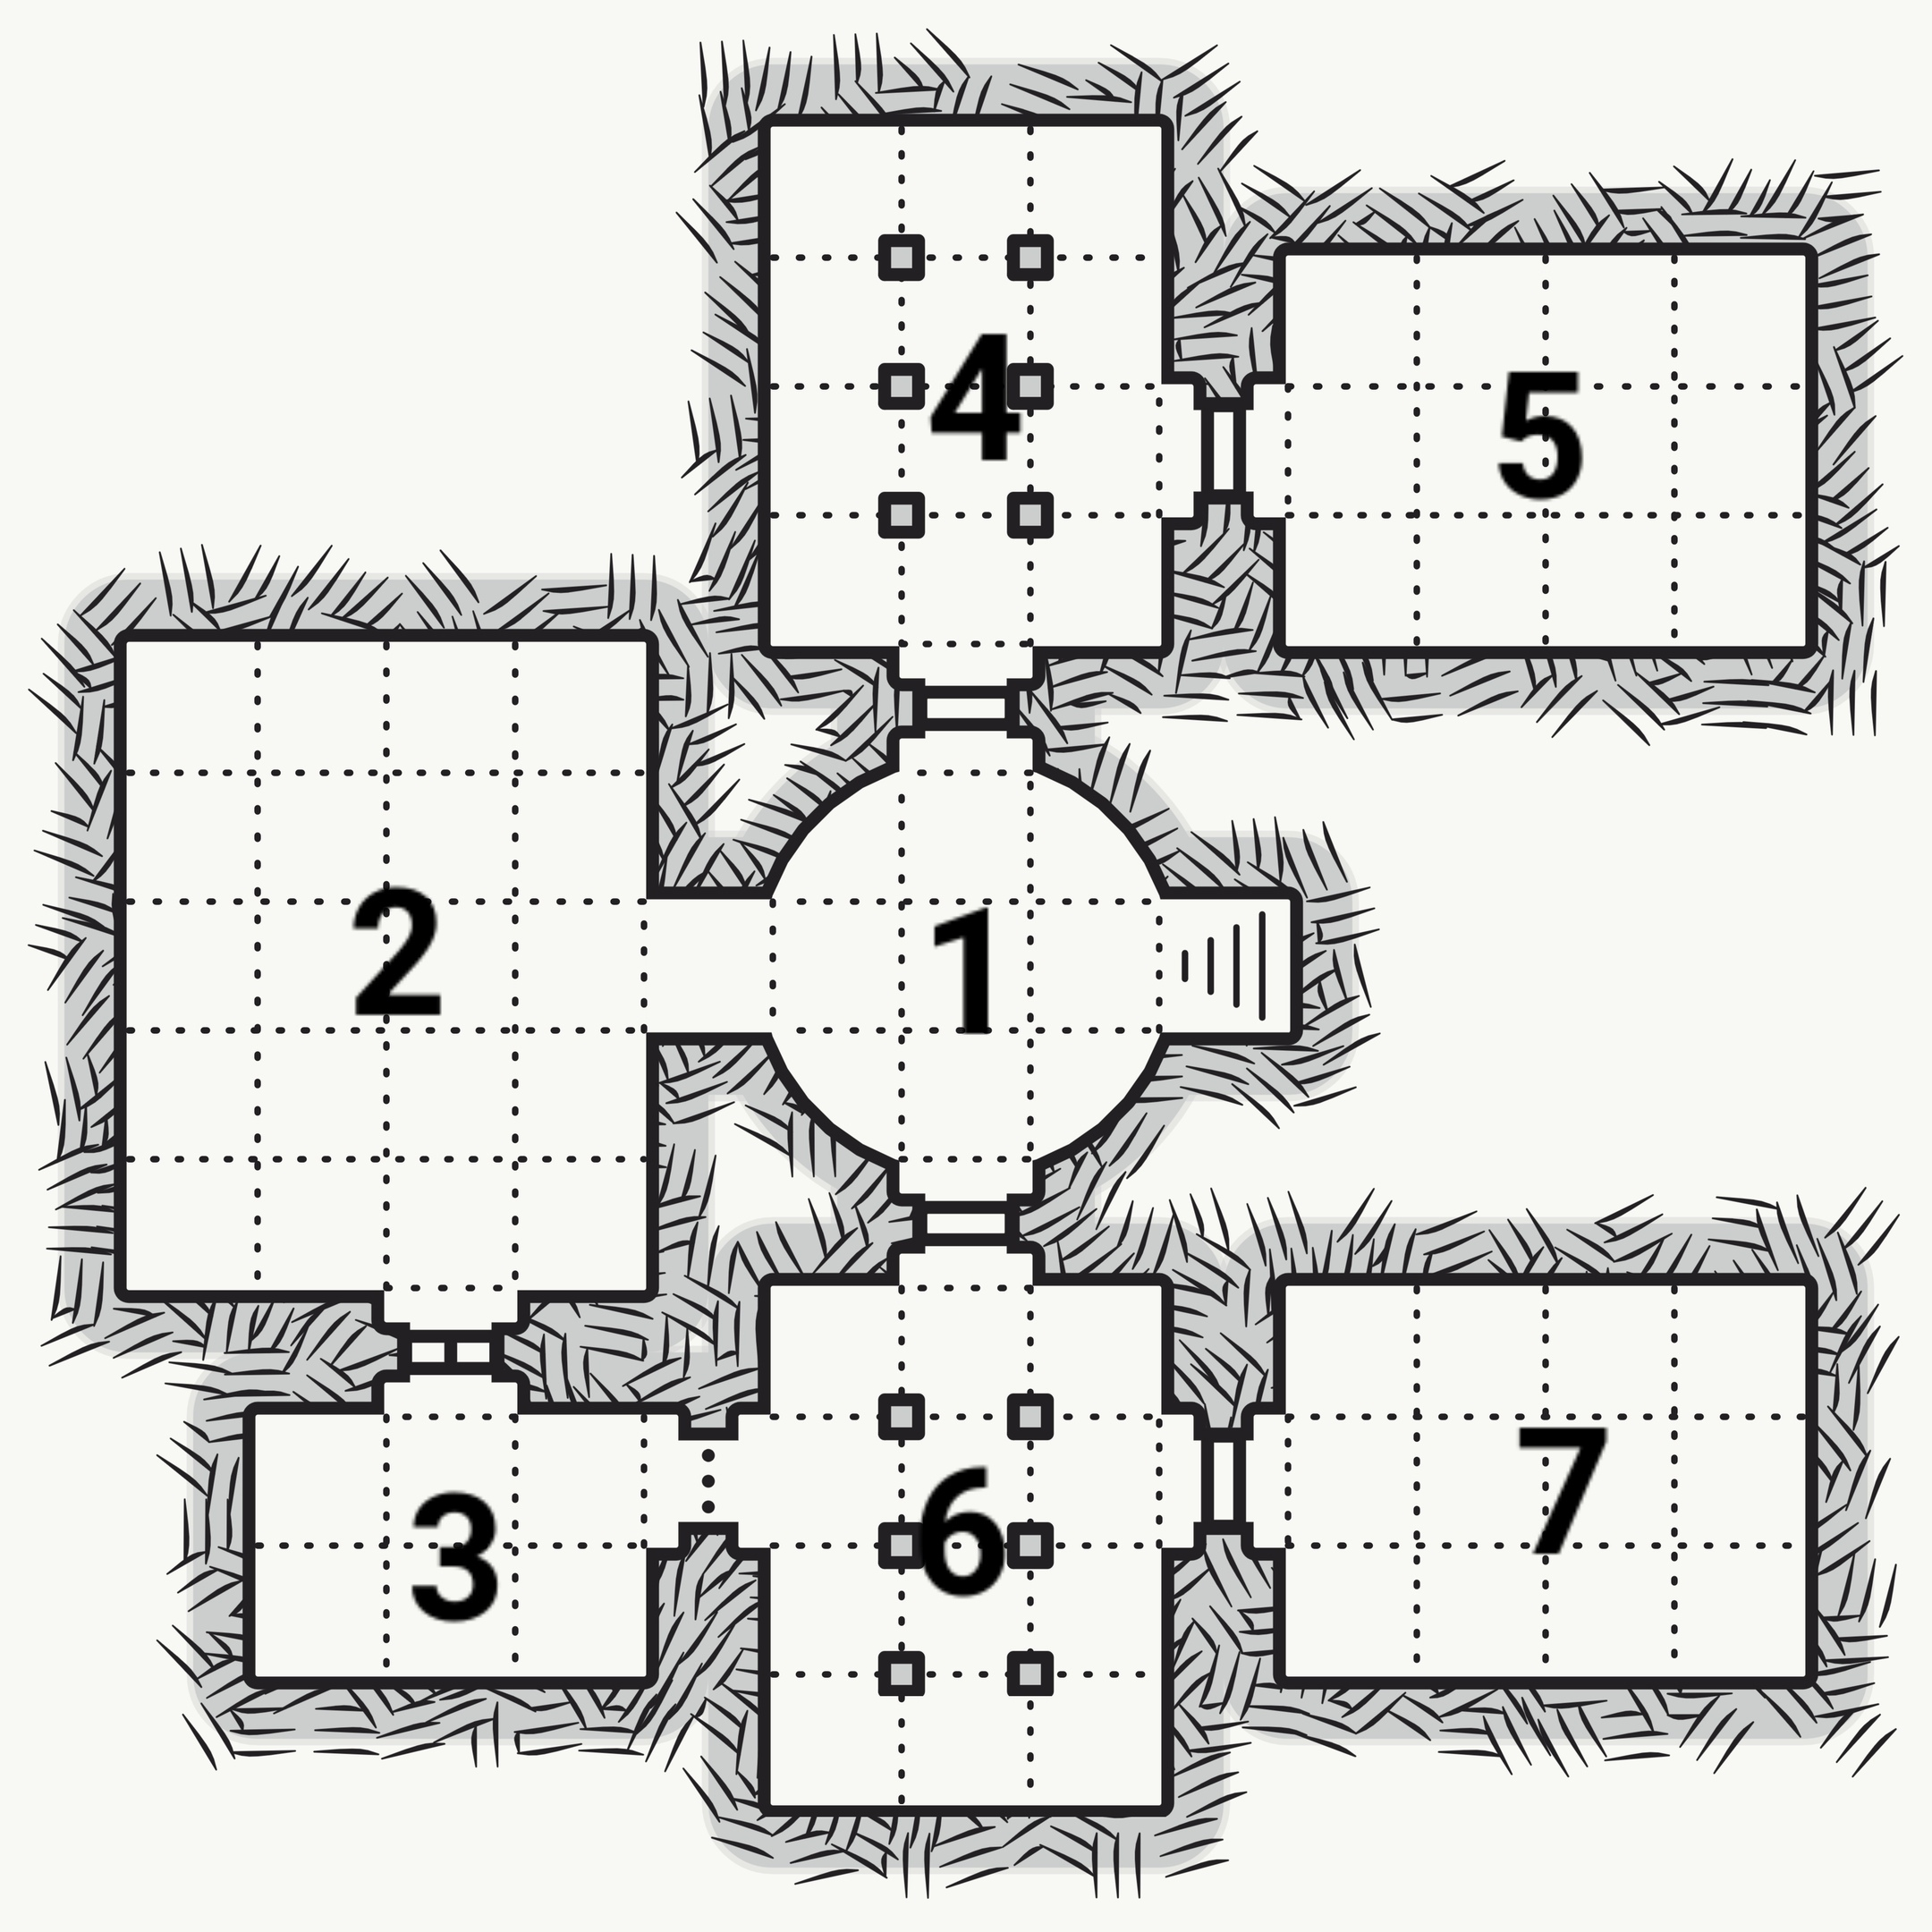
\includegraphics[width=0.5\textwidth]{3}

\begin{enumerate}
\item Круглая комната, по бокам двери, впереди открытый проход
\item Справа стоит стол, в него воткнут мясницкий нож. На столе лежат полугниющие куски мяса и пара практически пустых склянок с жидкостью. Запах стоит ужасный. В углу котелок на огне. INT CHECK: это мясо явно не животного
\item Железная дверь, закрыта намертво. PER: в внизу небольшой засов. Внутри тихо, нифига не видно. когда игроки будут отходить раздастся негромкий железный звук
\item Деревянная дверь на простом замке. Стены обрамляют колонны, меж них горки костей. На стене размазанная надпись углем "они его съели". ENCOUNTER: 2 скелета
\item Дверь на засове, закрыта с этой стороны. Посередине комнаты лестница наверх. В потолке люк, если приподнять его то оказываешься в комнате таверны.
\item Дверь из круглой комнаты открыта. Ящики с одеждой ==== Первое что вы видите, это человека в темной робе со свечкой в руке, но запирает за собой дверь. ==== получив удар он побежит в сторону к решетке, по пути надавив на колонне камень, и кинет факел за опускающуюся решетку. накиданыне чуваки помогут ему в бою. ENCOUNTER: 1 cultis + 3 slow bodies 
\item Факелы по сторонам, лестница вниз высокий потолок. PER CHECK: на полу 2x2 выступ,  на потолке шипы, на стене у лестницы рычаг, опущен вниз. TRAP: если рычаг поднят, ловушка активна. чувак которого они видели выше выключил ловушку.
\end{enumerate}

\subsection{4: Quarters}
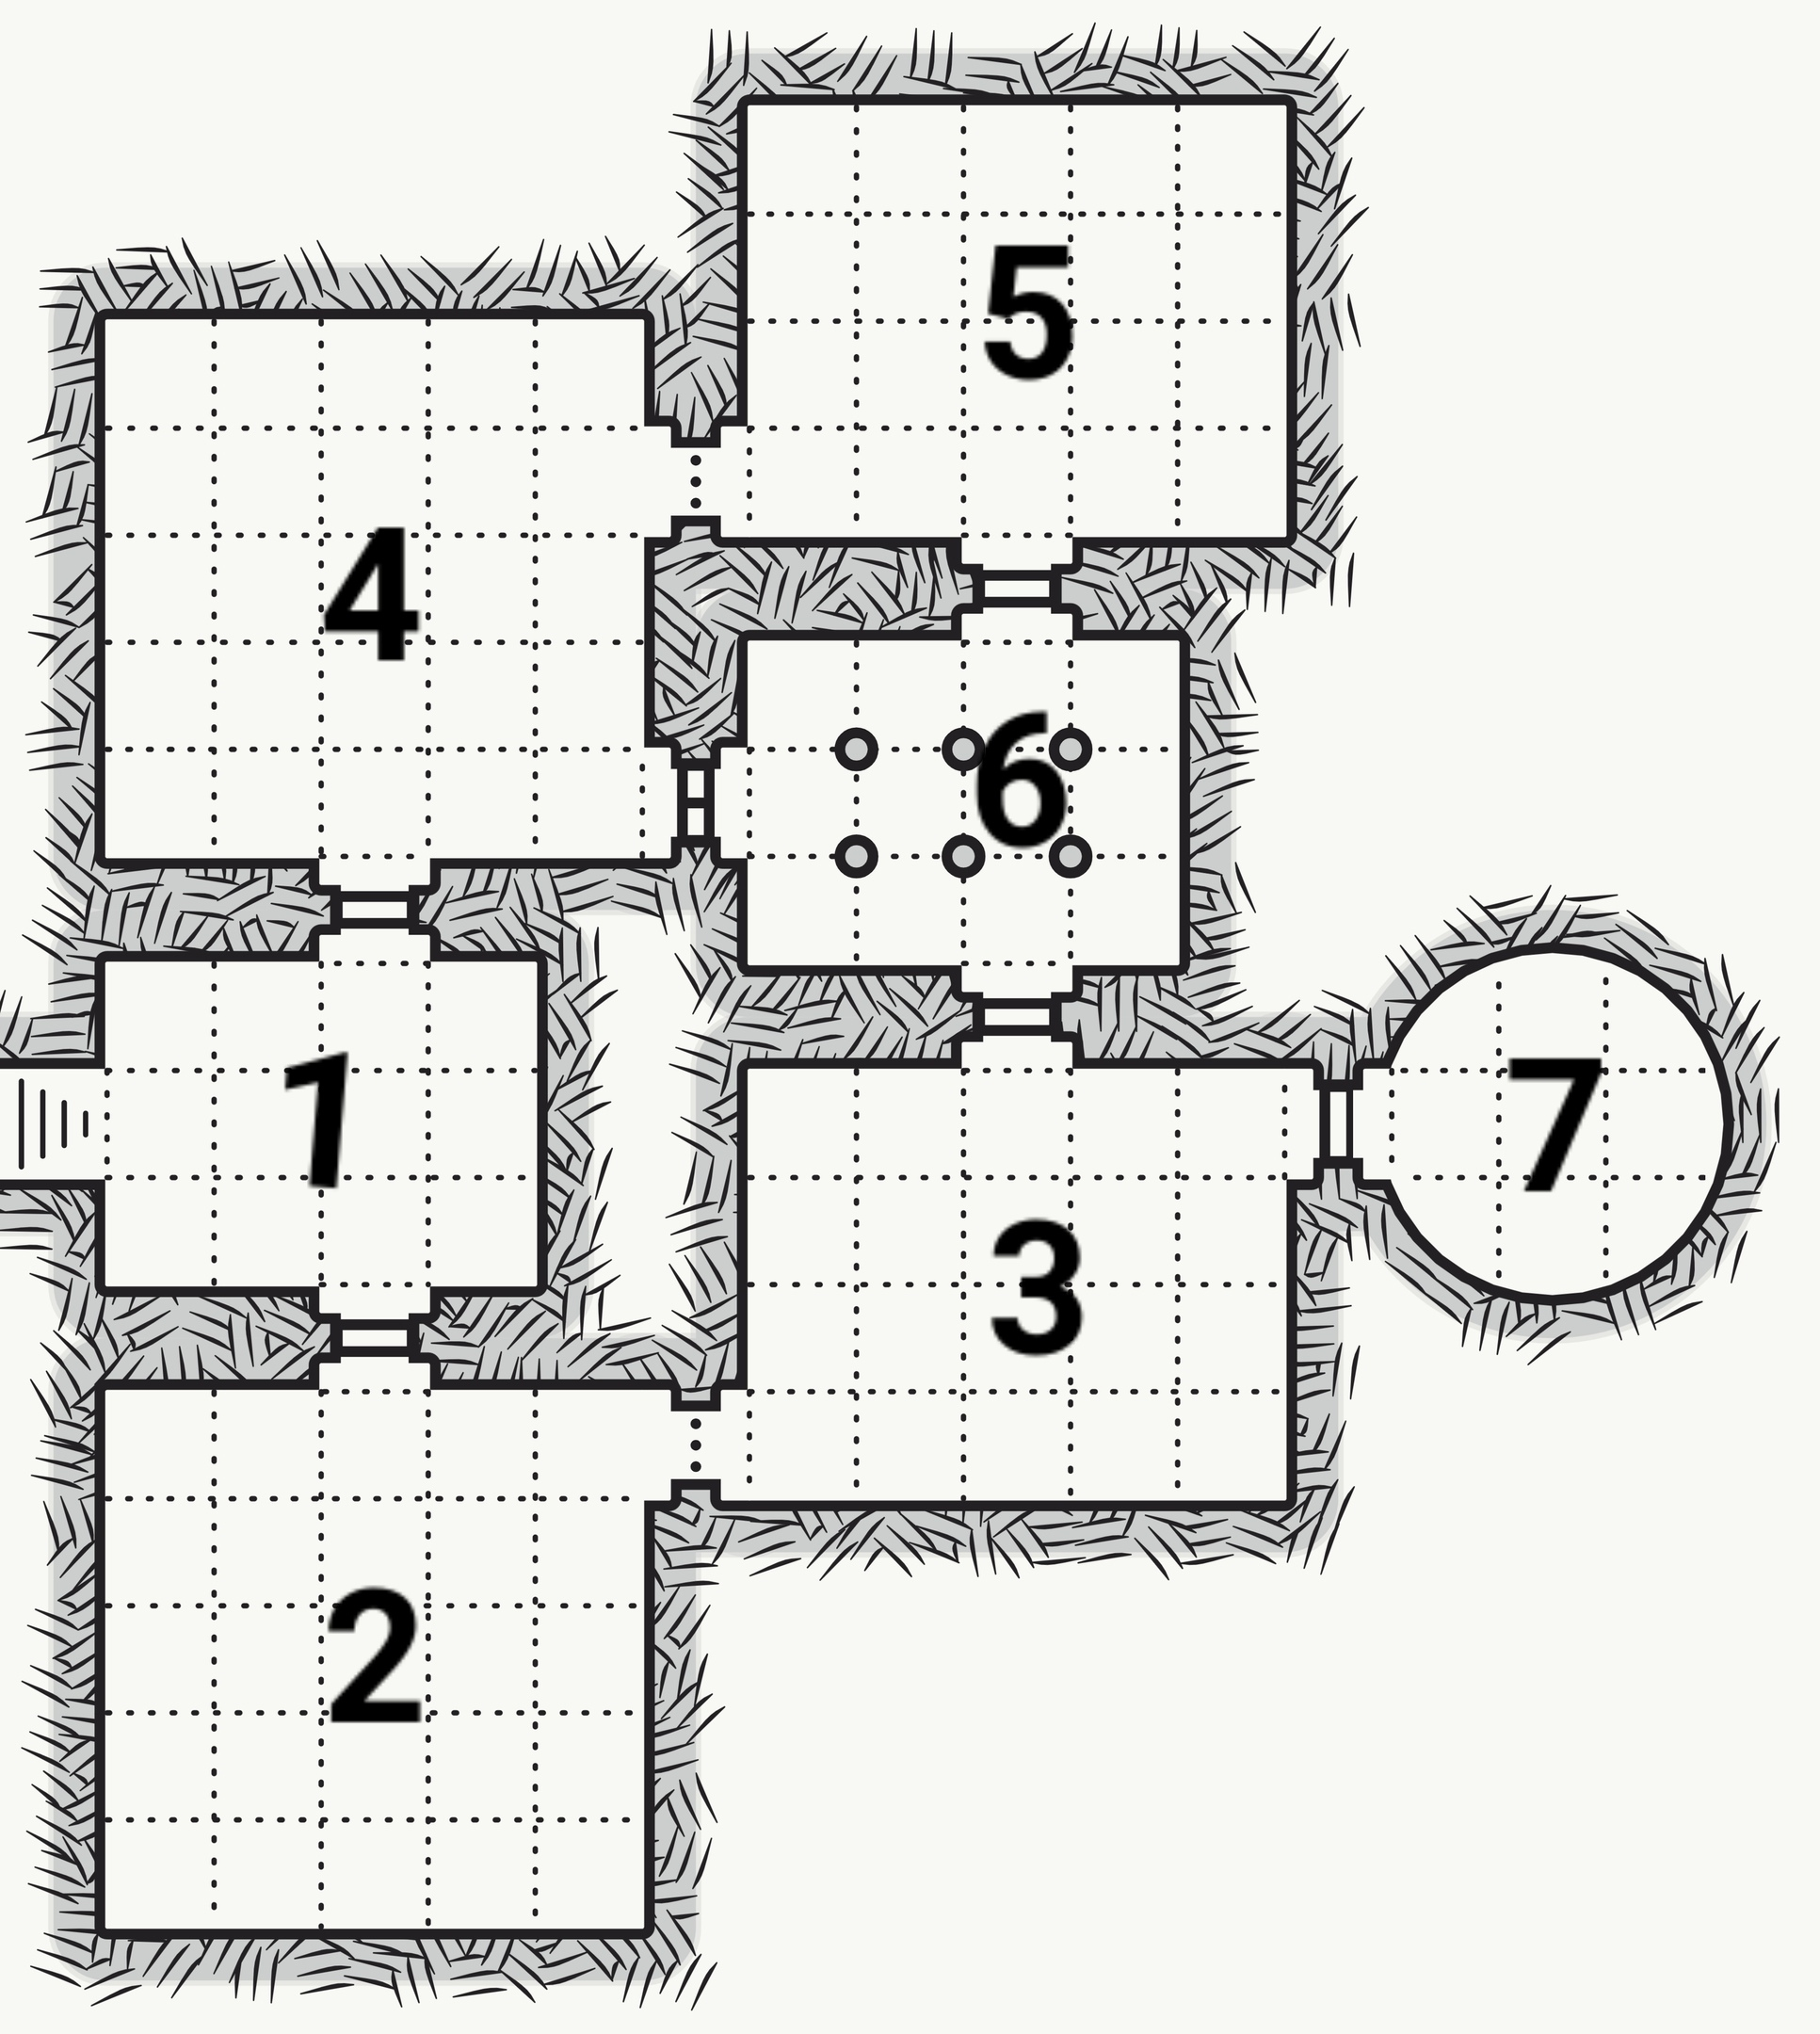
\includegraphics[width=0.5\textwidth]{4}
\begin{enumerate}
\item Напротив лестницы стул, на нем стоит свечка, лежит книга и миска с едой. PER: еда горячая, кто-то скоро вернется чтобы ее съесть. Он выходит из 4 не замечая групу.
\item Дверь закрыта. Перед железной решеткой стоит кресло. На другой стороне лестница вниз. У кресла стол, на столе кружка литра так на три-четыре. PER: кресло обито стершимся, но тонкой работы красным бархатом. -- За решеткой начинают читать в несколько голосов что-то на непонятном языке.
\item Проходит ритуал. Весь пол исчерчен символами. Четверо темных фигур стоят вокруг жертвы. Один из них подходит к жертве и вонзает кинжал в ее грудь кинжал. Он отходит. Отальные не прекращая чант берут тело за руки и ноги и тащать в соседнюю комнату.
\item Дверь открыта. Расставлены деревянные столы и стулья, кровати с идентичными матрасами. Несколько человек спит, один повернут к вам спиной, он готовит.
\item Кладовка. ящики с травами, ткани, алкоголь. В некоторые было беспорядочно скинуто разное барохло (вещи жертв)
\item По сторонам комнаты стоят стелажи с книгами, по середине стол.
\item В центре круглой комнаты яма вниз, запах из нее ужасный. На полу кровавый след ведущей к ней.
\end{enumerate}

\pagebreak

\subsection{5: Reception}
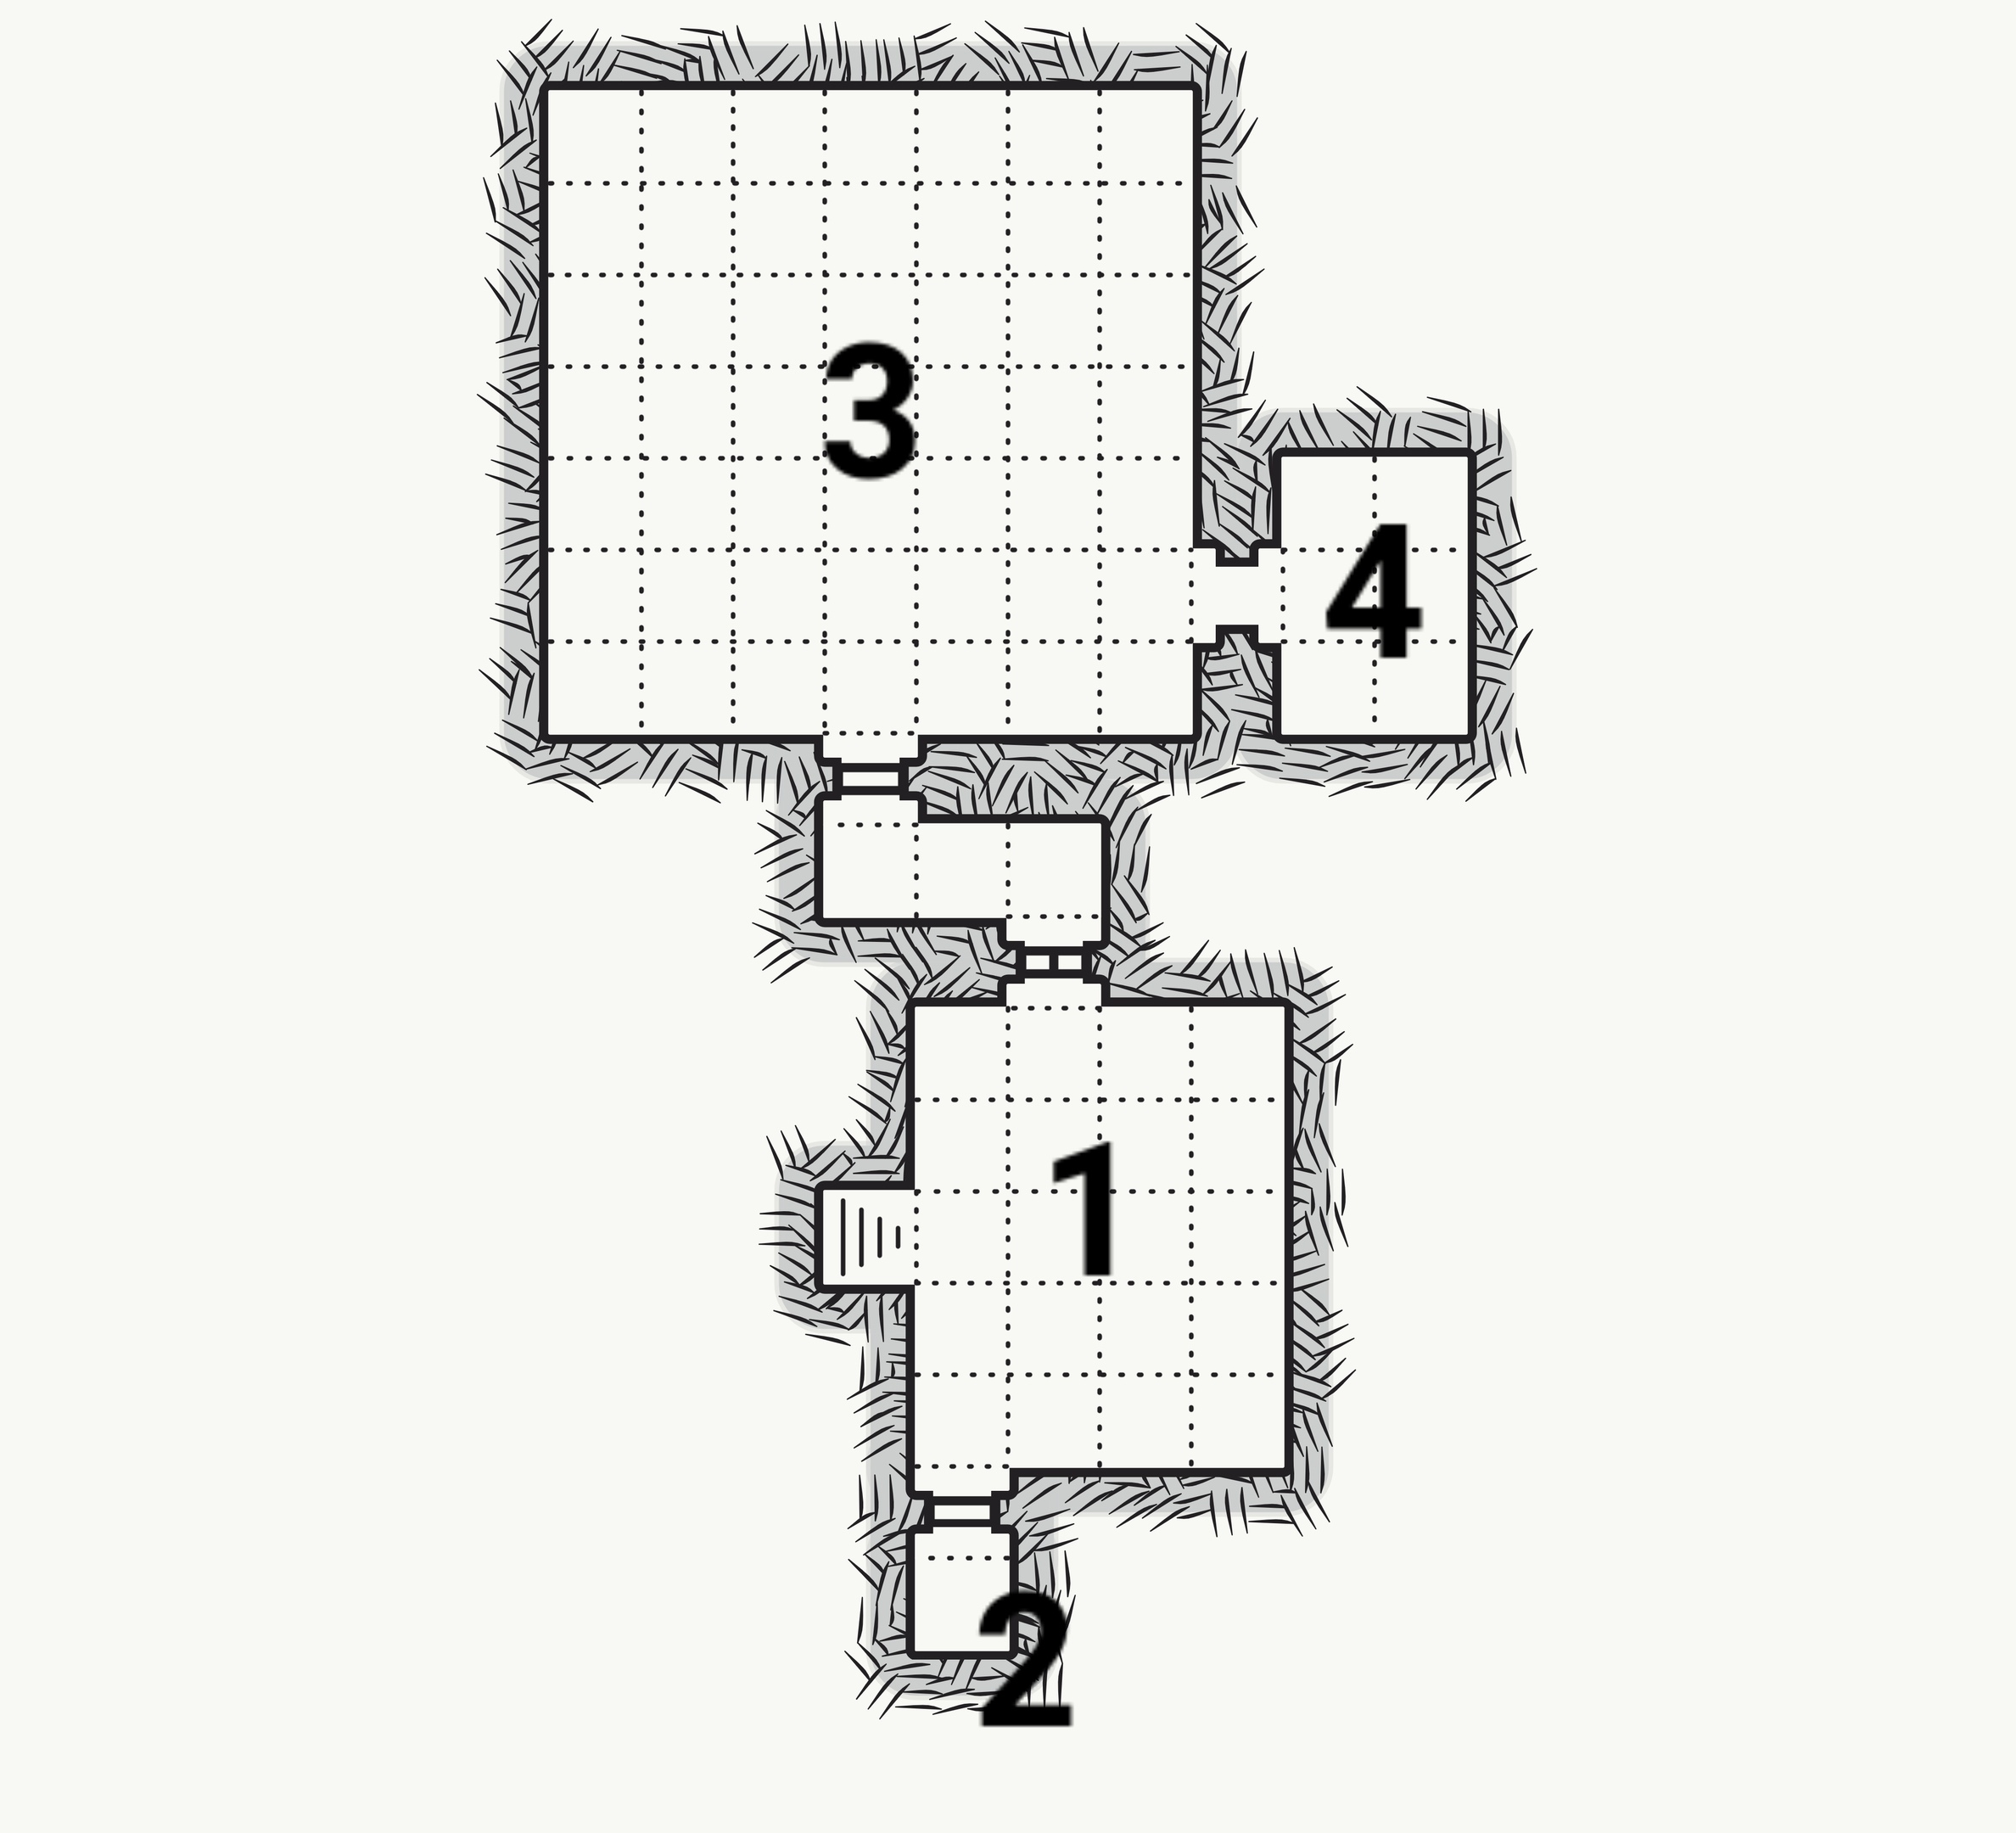
\includegraphics[width=0.5\textwidth]{5}

\begin{enumerate}
\item Первое что бросается в глаза, это то что тут убрано. Чисто. Впереди стоит диван, перед ним столик с книгами. Справа от входа небольшая дверь, слева стоит стол, за ним сидит скелет, когда вы входите он поднимает на вас взгляд. PER: Скелет слегка мерцает. Над ним вывеска с какой-то надписью INT: это не обычная некромантия. Надпись: "секретарь"

\begin{boxed}
Брат сейчас занят. Но если это что-то срочное, я могу пойти разбудить.
\end{boxed}

\item Кладовка, в ней метла. Скелет предупреждает, "я бы ее не трогал". TRAP: метла живая, улетает и уворачивается если по ней замахнуться, бьет по лицу, а потом возвращается на место
\item большое помещение, весь пол устлан костями, так, что его не видно. по комнате расставлены свечи и образуют круг. Посередине на возвышении стоит трон, рядом с троном небольшой круглый стол на высокой ножке. На столе огромных размеров золотой кубок. PER: в нем эль. INT: ты чувствуешь потоки магии тянущиеся к кубку откуда-то сверху.
\item Раздается скрежет, а потом резкий звук как будто на камень упало что-то тяжелое. Огромный скелет появляется из мрака в сопровождении скрежета обломка меча, который он устало тащит за собой. Игнорируя вас, он подходит к столу, берет кубок, делает пару глотков. 

\begin{boxed}
Я смотрю у нас гости?

-- who are you -- Да так, две груды костей что решили проведать старых друзей. 

-- what are you doing -- дарую людям забвение и лучший эль что они когда либо пили. а взамен забираю их чувства, мечты, память. *покручивает в руке кубок*

-- why? -- нет связующей силы более надежной чем та, что вбирает в себя души людские. я подарю брату жизнь которой у него никогда не было

Но хватит пустой болтовни. *со звоном на каменный пол он бросает свой кубок* Ваше приключение подходит к концу. 

Договорив это он откидывает нижнюю челюсть и из его рта валит черный дым, распространяется быстро и тушит свечи одну за другой. В воцарившейся тьме зеленым цветом переливаются его кости.
\end{boxed}

his body will stop glowing after a couple of turns

he will raise a bunch of very weak skeletons filled with memories he consumed

he can swap consciousnesses for a turn or two or mix them together ?

\end{enumerate}

% }}}











\end{multicols}

\end{document}

\subsection{Descent}
by now the party should be hooked and swarm the well. have them dive into water one way or another (roll endurance checks for suffocation, maybe make it just a bit dramatic)

the party emerges in the beginning of what looks like an old ruin/dungeon. the place is pretty humid, moss everywhere, rats squeaking somewhere, very dark.

glowing and regular mushrooms, the regular ones are piosonous

\subsection{Dungeon}
pack a bunch of e. a. poe into this. same kind of gothic unsettling horror with a tinge of madness (think cask of amontillado and the pit and the pendulum)

the layout should be separated into floors (4+boss arena?) that get more and more dangerous and typical fantasy-ish. things progress from just rats, to animated skeletons, to traps, to cultists.

room/encounter ideas:
\begin{enumerate}
  \item a door that players need to push together to open
  \item some stupid animated thing like a broom or something that fights them
  \item a trap room that fills with water (yes, that water) to the ceiling in a few turns
\end{enumerate}

\subsection{Interrogation}
around half way through the players may capture a cultist and interrogate him. tell them some stuff about the final boss (section below).

\section{Act III}
\subsection{Final Boss}
make it some large skeleton with glow in the dark bones. this ancient dude is some kind of a demigod that the cultists worship.

have it be a gimicky-ish bossfight where becomes visible/attackable for a turn after you shine light onto him, and then fades away and becomes invisible/invincible. also he's invisible if there's any light around.

when the party enders the room have the lights on, once the combat starts he breaks the torches and they see the green glow, next turn he fades.

let's say that he hasn't regained his physical form yet, and he needs souls to get it back and that's his motive. also he likes getting drunk? scratch that, makes him too likeable.

\subsection{Reveal}
the cultists perform rituals that poison the water in the well, making the water take VERY GOOD and take the souls of those who drink it. the souls are then fed into skeleton and make him more powerful



%===
%
%Хозяин таверны вернулся за стойку. "О, посетители? Чего желаете? Комнату? Выпить?"
%
%\textbf{per low} На ней стоит почти выпитая кружка эля.
%\end{boxed}
%
%if the players rent a room, have time pass weirdly, so that its the twilight again
%
%\subsection{Brewery}
%there's a black cat called Juro.
%
%if they go here first
%
%\begin{boxed}
%  составлена из бревен, внутри несколько человек. один перебирает зерно, двое других тоскают мешки, еще один размешивает что-то в чане. вокруг стоят уже закрытые бочки
%\end{boxed}
%
%if they go here after the tavern:
